\documentclass[12pt,journal,a4paper,twoside,onecolumn]{IEEEtran}
\usepackage{amssymb}
\usepackage{mathtools}
\usepackage{ amsmath, bm }
\usepackage{graphicx}
\usepackage{epstopdf}
\usepackage{yhmath}
\DeclareGraphicsExtensions{.pdf,.eps,.png,.jpg,.mps}
\usepackage{dsfont}
\usepackage{bbm}
\usepackage{setspace}
\usepackage[top=1.5in, bottom=1.5in, left=1in, right=1in]{geometry}

%For lemma, theorem, proposition, corllary, proof, definition,example and remark.
\newcommand{\rmnum}[1]{\romannumeral #1}
\newcommand{\Rmnum}[1]{\expandafter\@slowromancap\romannumeral #1@}
\makeatother

\newcommand\bigfrown[2][\textstyle]{\ensuremath{%
  \array[b]{c}\text{\scalebox{2}{$#1\frown$}}\\[-1.3ex]#1#2\endarray}}
% End
\author{An~Jiang,~
        Harry~Leib,~\\
          Department of Electrical Engineering\\
          McGill University\\
          Montreal,~Quebec,~Canada,~\\
          Email: an.jiang@mail.mcgill.ca,~harry.leib@mcgill.ca
}
\title{The Extended Neyman-Pearson Hypotheses Testing Framework and its Application to Spectrum Sensing in Cognitive Wireless Communication}
\date{\today}
\begin{document}
\begin{spacing}{2.5}
\maketitle
\begin{abstract}
Neyman Person (NP) testing for two hypotheses is widely used in radar system, spectrum sensing, medical detection and many other applications. Traditional NP testing maximizes the probability of detection under a probability of false alarm constraint. This paper consider an extended form of the NP test that is suitable for spectrum sensing when there might be different type of primary signals.
\end{abstract}

\begin{IEEEkeywords}
Neyman Pearson, Hypothesis Testing, Spectrum Sensin, Cognitive Radio
\end{IEEEkeywords}

\section{Introduction}
The increasing radio spectrum demand for wireless communication is driving the development of new approaches for its usage, such as Cognitive Radio (CR)\cite{a001}. The concept behind CR networks is the unlicensed use of radio spectrum while ensuring no interference to the licensed users. \cite{goldsmith2009breaking}.
To achieve this goal, a CR system must have ``cognitive" abilities to identify opportunities for communication\cite{buddhikot2007understanding}. In CR systems, the spectrum sensing component brings in such capabilities \cite{tandra2009spectrum}.

 Spectrum sensing has been a subject for extensive studies in the last years\cite{axell2012spectrum}. Common techniques for spectrum sensing are based on energy detection, exploitation of cyclostationarity properties of  the signal being sensed, and also could use preamble sequences that are embedded in the signals \cite{cabric2004implementation}.  In \cite{axell2011optimal}, the authors point out that for OFDM signals when the variances of the noise and signal are known, the performance of energy based spectrum sensing is very close to optimal. Cooperative spectrum sensing \cite{ganesan2005cooperative}, employing multiple sensors that are geographically scattered, are effective against shadowing.
Different sensing algorithms and DSP techniques have been introduced for specific situations, such as in \cite{tian2007compressed} where the authors study algorithms for wide band spectrum sensing focusing on sub-Neyquist sampling techniques. In  \cite{sun2013wideband} and  \cite{sun2013wideband2} the authors propose compressed sensing and sub-Nyquist sampling techniques for wide band spectrum sensing.

In order to detect a free frequency channel, a spectrum sensing scheme solves a binary hypotheses testing problem, where the null hypothesis refers to the event that a user is not using the channel and the alternative hypothesis refers to the event that a user is occupying the channel. If the a-prior probabilities of null and alternative hypotheses are known, then such a problem can be solved using a Bayesian framework \cite{poor1994introduction}. The situation when Baysian framework could be used is considered in \cite{zeng2010review} and the performance of such scheme is analyzed.
Even though the Baysian framework can be used in some situations, in more often cases, the a-prior probabilities are not available. In such situations Neyman Pearson testing is employed \cite{poor1994introduction}.When there is a single type of primary user (two hypotheses), NP testing will achieve the largest probability of detecting a vacant channel when no primary user is present under a constraint on the probability that the channel will be declared vacant when in fact a primary user is present.
Traditional NP testing has been extensively used for two hypotheses problem. In such cases,  the performance is characterized by the Receiver Operating Characteristic (ROC) curve, which represents the relationship between probability of detection and probability of false alarm \cite{poor1994introduction}.

In spectrum sensing application, there may be more than one type of primary users. For example in IEEE 802.22 \cite{shellhammer2008spectrum} the channel can be occupied by Analog-TV Digital-TV and wireless microphone. In such cases, an extended NP (ENP) test can provide important advantages \cite{zhang1999desig}. A detector based on ENP testing can ensure the largest probability of detection under a separate constraint of false alarm for each primary user type \cite{LehmannTest}.

With an ENP detector however, the achievable false alarm probabilities are limited. In this work we analyze the properties of the ENP test and propose the Modified Extended Neyman Pearson (MENP) test, that circumvents the limitations of the false alarm probabilities. The structure of the remaining of this paper is [TO BE ADDED].

\section{Extended Neyman Pearson Test}

\subsection{Introduction to Extended Neyman Pearson Test}
The theories of hypotheses testing have been a subject of continuous studies, and have found applications in various fields such as radar systems, spectrum sensing for cognitive communication systems, and in  medical science. One type of hypotheses testing problem can be abstracted as  follows: assume $M+1$  hypotheses $H_0$, $H_1$, ..., $H_{M}$, inducing $M+1$  Probability Density Functions (PDFs) on the observable $Y$.

  \begin{equation}
\label{equ:hypothesis}
\begin{split}
H_0:\;\;\;\;\;\;\;\;\;&Y \sim f_0(y) \\
H_1:\;\;\;\;\;\;\;\;\;&Y \sim f_1(y)\\
&......\\
H_M:\;\;\;\;\;\;\;\;\;&Y \sim f_M(y)\\
\end{split}
\end{equation}
Based on $y$, a realization of $Y$, the detector needs to decide whether or not it comes from $f_0(y)$. A framework for solving this problem for $M=1$ was introduced in \cite{neyman1933problem} and it is commonly known as Neyman Pearson (NP) testing. The theory of NP testing was further developed in \cite{wald1939contributions}. In \cite{dantzig1951fundamental}, the theory of NP testing was  expanded also for $M>2$. A comprehensive exposition of such generalized NP testing can be found in \cite{LehmannTest}.

\noindent  \textbf{The Extended Neyman Pearson (ENP) Lemma:}
\textit{
Let $f_0(x), f_1(x), ..., f_{m}(x)$ be real Borel measurable functions  defined on finite dimensional  Euclidean space $\mathcal{R}$ such that $\int \limits_R | f_i(x)|\mathrm{d}x < \infty (i=0, 1,...,M)$.  Suppose that for given constants $c_1,...,c_M$ there exists a class of subsets $\mathcal{S}$, denoted $\mathcal{C}_\mathcal{S}$, such that for every $\mathcal{S} \in \mathcal{C}_\mathcal{S}$ we have
\begin{equation}
\label{one}
\int\limits_\mathcal{S} f_i(x)\mathrm{d}x = c_i, \;\;\;\;\;\;i=1,...,M
\end{equation}
Then:
%No. 1
\\\textnormal{(\rmnum{1})} Among all members of $\mathcal{C}_\mathcal{S}$ there exists one that maximizes
\[
\int \limits_\mathcal{S} f_{0}(x)\mathrm{d}x.
\]
%No.2
\\\textnormal{(\rmnum{2})} A sufficient condition for a member of $\mathcal{C}_\mathcal{S}$ to maximize
\[
\int \limits_\mathcal{S} f_{0}(x)\mathrm{d}x.
\]
is the existence of constants $k_1,...,k_M$ such that
\begin{equation}
\label{2}
f_{0}(x)>\sum\limits_{j=1}^M k_j f_j(x)\;\;\;\;\text{when $x \in \mathcal{S}$}
\end{equation}
\begin{equation}
\label{3}
f_{0}(x)<\sum\limits_{j=1}^M k_j f_j(x)\;\;\;\;\text{when $x \notin \mathcal{S}$}
\end{equation}
%No. 3
\\\textnormal{(\rmnum{3})} If a member of $\mathcal{C}_\mathcal{S}$ satisfies  \textnormal{(\ref{2})} and \textnormal{(\ref{3})} with $k_1,...,k_M\geq0$, then it maximizes
\begin{equation}
\label{4}
\int \limits_\mathcal{S} f_{0}(x)\mathrm{d}x
\end{equation}
among all $\mathcal{S} \in \mathcal{C}_{\mathcal{S}}$ satisfying
\begin{equation}
\label{5}
\int \limits_\mathcal{S} f_i(x)\mathrm{d}x\leq c_i,\;\;\;\;i=1,...,M.
\end{equation}
}

The associated probability of detection, $P_d$ and false alarms $P_{f_i}$ for a certain subset $\mathcal{S}$ are defined as \cite{neyman1933problem}, $P_d = P(H_0 | H_0) = \int_{\mathcal{S}}f_0(x)\mathrm{d}x, P_{f_i} = P(H_0 | H_i) = \int_{\mathcal{S}}f_i(x)\mathrm{d}x\;\; i = 1, ..., M $. Define the step function

\begin{equation}
   \label{equ: step function}
   u(x) = \begin{cases}
     0\;\;\;\;\;\;&x < 0\\
     0.5\;\;\;\;\;\;&x=0\\
     1\;\;\;\;\;\;&x>0\,,
   \end{cases}
\end{equation}
Then for a subset $\mathcal{S}$ satisfying \eqref{2} and \eqref{3} we have:
\begin{equation}
\label{equ: pf and pd}
\begin{split}
&P_d = \int_{-\infty}^{\infty} u(f_0(x) - \sum_{j=1}^{M}k_jf_j(x)) f_0(x)\mathrm{d}x	\,, \\
&P_{f_i} = \int_{-\infty}^{\infty} u(f_0(x) - \sum_{j=1}^{M}k_jf_j(x)) f_i(x) \mathrm{d}x\;\;	 i=1, 2, ..., M\,.
\end{split}
\end{equation}
The relationship between $P_d$ and $P_{f_i}$ can be represented by Receiver Operating Characteristic (ROC) surface \cite{LehmannTest}.

From to \eqref{2} \eqref{3}, the ENP Decision rule $\delta$ is

\begin{equation}
\label{equ: decision rule}
\delta: \sum_{j=1}^{M}k_j\frac{f_j(x)}{f_0(x)} \substack{H_0 \\ < \\ \geq \\ \bar{H}_0} 1
\end{equation}

From the  \textbf{ENP Lemma}, $\delta$  achieves the largest $P_d$ under the constraints $P_{f_i} = c_i (i = 1, 2, ..., M)$.
When $M=1$, it achieves the largest $P_d$ under the constraint $P_f \leq c$ \cite{LehmannTest}, which is the well known and commonly used form.

% notes from Prof. Leib.
For applications in spectrum sensing, $H_0$ denotes the hypothesis that the channel is free and $H_m \;(m=1, ..., M)$ corresponds to the hypothesis that the channel is occupied by the $m$-th primary signal. Although we have $M$ hypotheses, we intend to determine if the channel is free or not. Hence the problem is to find a binary test of deciding $H_0$ versus $\bar{H}_0$ such that $P_d$ is maximized under the constraints $P_{f_m} \leq c_m$ $m = 1, ..., M$. In context of spectrum sensing, $1-P_{f_m}$ can be interpreted as the protection level of the $m-$th primary signal. The larger is this protection level, the smaller is the probability that when the $m-$th signal is active, the test will not detect it and will declare the channel free. In context of spectrum sensing the solution of the ENP problem maximizes the probability of detecting a free channel under a constraint on the protection level for each primary signal. The protection levels of primary signals can be different and they are guaranteed.

\subsection{Properties of Extended Neyman Pearson Test}
We consider now several properties for the ENP test, embodied by three lemmas with proof placed in the appendix A, B and C.

\noindent \textbf{Condition 1}
\textit{
\noindent Let $f_i(x) \;\;i=0, 1, ..., M$ be the PDF induced by hypothesis $H_i$, and define $g(x) = f_0(x) - \sum_{j=1}^{M} k_jf_j(x)$ where $k_i$  ($i = 1, 2, ..., M$) are real numbers. Let $\mathcal{D} \in \mathbb{R}$ be an open set such that $\int_{\bar{\mathcal{D}}}f_i(x)=0\;\;i = 1, 2, ..., M$. Furthermore,  if $x_0$ is a solution  for $g(x) = 0 \;\;(x \in \mathcal{D})$, there exists an integer $n$ such that  the $n$ order derivative of $g(x_0)$ is not equal to zero $(g^{(n)}(x_0) \neq 0)$.
}

\noindent \textbf{Lemma 1}
\textit{
\noindent Under}
\textbf{Condition 1}
\textit{, let $\mathbf{P}$ be a point with coordinate $(P_d, P_{f_1}, ..., P_{f_M})$ on the ROC surface of the EPN test. If there exists a tangent hyperplane at $\mathbf{P}$, then its normal is parallel to the vector $\mathbf{n} = (-1, k_1, ..., k_M)$, where $k_i$ are the parameters of the ENP test achieving $\mathbf{P}$.
}

\noindent \textbf{Lemma 2}
\textit{
\noindent
Under}
\textbf{Condition 1}
\textit{, let $\mathbf{P}$ be a point on the ROC surface, $\frac{\partial P_d}{\partial P_{f_i}} \bigg|_P = k_i$, where $k_i$ are the parameters of ENP test achieving $\mathbf{P}$.
}

\noindent \textbf{Lemma 3}
\noindent \textit{
    Let $f_0$, $f_1$, ..., $f_M$ be PDFs defined on set $\mathcal{D}$ and suppose that for given constants $c_1, ..., c_M \in (0, 1]$ there exists a critical function $\phi$ such that ${P}_{f_i} \leq c_i$ ($i=1, ..., M$). Let $\mathcal{C}_\mathcal{S}$ be the set of critical functions satisfying ${P}_{f_i} \leq c_i$ ($i=1, ..., M$).
Then:
%No. 1
\\\textnormal{(\rmnum{1})} Among all members of $\mathcal{C}_\mathcal{S}$ there exists one that maximizes $P_d$.
%No.2
\\\textnormal{(\rmnum{2})} If $f_i(x) \neq 0$ holds a.e. $\mathcal{D}$ ($i=0, 1,..., M$), and $\phi^{\ast}$ is a member of $\mathcal{C}_\mathcal{S}$ that maximum $P_d$, then there exists non-negative constants $k_1, ..., k_M$ such that 
\[
\phi^\ast(x)= 1\;\;\;\;\textit{if}\;\;\;\;f_0(x) > \sum_{i=1}^{M}k_if_i(x)
\]
\[
\phi^\ast(x)= 0\;\;\;\;\textit{if}\;\;\;\;f_0(x) < \sum_{i=1}^{M}k_if_i(x)
\]
holds a.e. on $\mathcal{D}$.
}

\subsection{Modified Extended Neyman Pearson Algorithm}
%define \JUDGEMENT
\def \JUDGEMENT{u(f_0(x) - \sum_{j=1}^{M}k_j f_j(x))}
Before we proceed, we will define some notations for presentation.
Define $\mathbf{c}^T = [c_1, c_2, ..., c_M]$, $\mathbf{a}^T=[a_1, a_2, ..., a_M]$, $\mathbf{k}^T = [k_1, k_2, ..., k_M]$ and  $\mathbf{P}_f^T = [P_{f_1}, P_{f_2}, ..., P_{f_M}]$. Let
$F(\mathbf{a})$ denote the largest $P_d$ under the constraints $P_{f_i} = a_i\;\;i = 1, ..., M$.
$G(\mathbf{c})$ denote the largest $P_d$ under the constraints $P_{f_i} \leq c_i\;\;i = 1, ..., M$.
Also define the set $\mathcal{A}_\mathbf{c} = \{
  \mathbf{P}_f | 0 \leq P_{f_i} \leq c_i
  \;\;i=1, 2, ..., M\}\,.
$ and set $\alpha^+ \triangleq \{\mathbf{P}_f | P_{f_i} = \int_{-\infty}^{\infty} \JUDGEMENT f_i(x) \mathrm{d}x, \text{where\;\;} k_i \geq 0 \;\;i=1, ..., M\}$.
Let $\mathbf{A}$ and $\mathbf{B}$ denote two vectors. 
By $\mathbf{A} \leq \mathbf{B}$, $\mathbf{A} = \mathbf{B}$ and  $\mathbf{A} \geq \mathbf{B}$ we mean that every element of $\mathbf{A}$ is no larger than, equal to and no smaller than its corresponding element of $\mathbf{B}$, respectively. 

In practice (e.g. spectrum sensing in CR communication system), the following problem needs to be solved,

      \begin{equation}
      \label{equ: problemstate}
      \begin{split}
      \max\;\;\;\;\;\;&P_d\\
      \text{s.t.}\;\;\;\;\;\;&\mathbf{P}_f \leq \mathbf{c}
      \end{split}
      \end{equation}

According to ENP Lemma, this problem can be solved by an ENP test only when there are parameters $k_i \geq 0, \;\;i=1, ..., M$ such that 
\begin{equation}
\label{equ: condition for ENP}
\begin{split}
c_i = \int_{-\infty}^{\infty}u(f_0 - \sum_{j=1}^{M}k_jf_j(x))f_i(x)\mathrm{d}x \;\;i = 1, ..., M
\end{split}
\end{equation}

The case when the given $c_i\;\;i = 1, 2, ..., M$ do not satisfy \eqref{equ: condition for ENP} was not considered so far. 

Next we present the Modified Extended Neyman Pearson Test (MENP) for solving \eqref{equ: problemstate}.

\noindent \textbf{Modified Extended Neyman Pearson Test}
\noindent \textit{
\\\textnormal{(\rmnum{1})} Assume $\mathbf{c} \in \alpha^+$. Then there must be a $\mathbf{k}^0 = [k_1^0, k_2^0, ..., k_M^0]^T$ with $k_i \geq 0\;\;i=1, ..., M$ satisfying
}
\begin{equation}
\label{equ:Pf}
  P_{f_i}^0 = \int_{-\infty}^{\infty} u(f_0(x) - \sum_{j=1}^{M}k_j^0f_j(x))f_i(x)\mathrm{d}x = c_i \;\; (i= 1, 2, ..., M)\,.
\end{equation}
\textit{
    and the decision rule $\delta $ solving  \eqref{equ: problemstate} is:
}
\begin{equation}
\label{equ:decision rule}
\delta:\;\;\;\;\frac{f_0(x)}{\sum_{i=1}^{M}k_i^0f_i(x)} \substack{H_0 \\ \geq \\ < \\ \bar{H}_0} 1
\end{equation}
\textit{
\noindent \textnormal{(\rmnum{2})} Assuming $\mathbf{c} \notin \alpha^+$, Let $\mathcal{C} = \mathcal{A}_{\mathbf{c}} \cap \alpha^+$, and $\mathbf{a}^0 = [a_1^0, a_2^0, ..., a_M^0]^T \in \mathcal{C}$ be such that
}
\begin{equation}
\label{equ: F0}
\max_{\mathbf{a} \in \mathcal{C}}\;\;\;\;F(\mathbf{a}) = F(\mathbf{a}^0)\\
\end{equation}
\textit{
Since $\mathbf{a}^0 \in \mathcal{A}_{\mathbf{c}} \cap \alpha^+$, from \textnormal{(\rmnum{1})} we have that there exists a vector $\mathbf{k}^0$ such that \eqref{equ:decision rule}  maximizes $P_d$ under the constraints $P_{f_i} = a_i^0, \;i=1, ..., M$. Here since $a_i^0 \leq c_i^0, \;i=1, ..., M$ this decision rule  solves \eqref{equ: problemstate}.
}

In Appendix D, we show MENP Test can provide an optimal solution for \eqref{equ: problemstate}.

Next we introduce a method of finding $\mathbf{a}^0$. For a specific $\mathbf{c}$, in order to get $\mathbf{a}^0$, we need to determine the set of $\alpha^+$. We can conduct an exhaustive search over a grid of $k_1, ..., k_M$ depending on the desired accuracy, and store these results ($P_d, \mathbf{P}_f, \mathbf{k}$) into a lookup table $T_1$. After that, we iterate every item in $T_1$ and put the item into table $T_2$ if the item satisfies:  $\mathbf{P}_f \leq \mathbf{c}$.
At last, we iterate every item in $T_2$ and get the largest $P_d$ and its decision rule $\mathbf{k}$.

\section{The ROC surface of MENP}

The ROC surface of MENP (M-ROC) depicts the relationship between $P_d$ and $c_1, c_2, ..., c_M$. On one hand, it  illustrates the largest $P_d$ can that can be achieved under the constraints $P_{f_i} \leq c_i (i = 1, 2, ..., M)$, on the other hand, it provides the range of $\mathbf{c}$ for a given $P_d$.
Points $(P_d, c_1, c_2, ..., c_M)$ on M-ROC  surface can be divided into two types: 
\\1. Those with $[c_1, c_2, ..., c_M] \in \alpha^+$. Define this set of points as $M_0$; 
\\2. Those with $[c_1, c_2, ..., c_M] \notin \alpha^+$. Define this set of points as $M_1$. 

Obviously points in $M_0$ can be achieved by MENP (\rmnum{1}) and points in $M_1$ can  be achieved by MENP (\rmnum{2}). Next we consider a property of the M-ROC surface.

\noindent \textbf{Property 1}
\noindent \textit{
  \noindent Assume hypotheses given as:
}
\begin{equation}
\begin{split}
H_0:\;\;\;\;\;\;&X \sim f_0(x)\\
H_1:\;\;\;\;\;\;&X \sim f_1(x)\\
  &......\\
H_M:\;\;\;\;\;\;&X \sim f_M(x)
\end{split}
\end{equation}
\textit{
  define $g(x) = \frac{\sum_{i=1}^{M}k_if_i(x)}{f_0(x)}$ and let $F_i(x)$ to represent the CDF of hypothesis $H_i$ ($i = 1, ..., M$). If $g(x)$ is a monotonically increasing function of $x$ for any non-negative $k_i\;\;(i = 1, ..., M)$ and $F_i(x)$ is monotonically increasing function, then we have:}
  
\textit{(1)The region achieved by ENP test with non-negative parameters degenerates to a curve and the decision rule for $M_0$ is $x \substack{\bar{H}_0 \\ \geq \\ < \\H_0} x_0$.}

\textit{(2)For a specific false alarm constraints $P_{f_i} \leq c_i\;\;(i = 1, ..., M)$, the decision rule for MENP test is $x \substack{\bar{H}_0 \\ \geq \\ < \\H_0} x_0$, where $x_0 = \min(F_1^{-1}(c_1), ..., F_M^{-1}(c_M))$.}

\textit{(3)The expression of $P_d$, $P_{f_1}$, ..., $P_{f_M}$ can be written as}
\begin{equation}
\label{equ: chi pd}
  \begin{split}
    P_d &= \text{Pr}(X \leq x_0 | H_0) = F_0(x_0)\\
        P_{f_1} &= \text{Pr}(X \leq x_0 | H_1) = F_1(x_0)\\
        &......\\
            P_{f_M} &= \text{Pr}(X \leq x_0 | H_2) = F_M(x_0)
  \end{split}
\end{equation}

The proof is given in the appendix E.

We consider two examples that illustrate the properties of M-ROC surface for $M = 2$.

\subsection{Gaussian Hypotheses}
Assume three hypotheses given as:
\begin{equation}
\label{equ: Gaussian Hypothesis}
\begin{split}
	H_0:\;\;\;\;\;\;\;\;&X \sim \mathcal{N}(-1,1)\\
    H_1:\;\;\;\;\;\;\;\;&X \sim \mathcal{N}(0,1)\\
    H_2:\;\;\;\;\;\;\;\;&X \sim \mathcal{N}(1,10)\,,
\end{split}
\end{equation}
where $\mathcal{N}(\mu,\sigma^2)$ denotes a Gaussian PDF with mean $\mu$ and variance $\sigma^2$.
To form the M-ROC surface, we first consider points in region $M_0$.The decision rule in region $M_0$ is given by \eqref{equ: decision rule}
with $M=2,\;\;k_1, k_2 \geq 0$, and the expression for $P_d$, $P_{f_1}$ and $P_{f_2}$ are given by \eqref{equ: pf and pd}. According to \textbf{Neyman Pearson Lemma}, if $k_1, k_2 \geq 0$, then $P_{f_1} = c_1$ and $P_{f_2} = c_2$.

We use Matlab to illustrate the region $M_0$. The values of $k_1$ and $k_2$ range from $0$ to $100$ in steps of $0.01$. Substituting the value of $k_1$ and $k_2$ into \eqref{equ: pf and pd}, results in the corresponding $P_d$ $P_{f_1}$ and $P_{f_2}$.  The set $M_0$ is illustrated in Figure \ref{pic: surface for m0 gaussian}. Figure \ref{pic: contour for m0 gaussian} presents the projection of Figure \ref{pic: surface for m0 gaussian} on the $c_1, c_2$ plane.
In Figure \ref{pic: contour for m0 gaussian}, region $N_0$ is the projection of region $M_0$ on the $c_1, c_2$ plane. Since $M_0$ is the set of points with $[c_1, c_2] \in \alpha^+$, $N_0$ is the region of points that belong to $\alpha^+$.
Define curve $L_1$ as the set of points that satisfy the conditions: (1) $(c_1, c_2) \in N_0$; (2) $(c_1, c_2+\epsilon) \notin N_0$, for any $\epsilon \geq 0$. Define curve $L_2$ as the set of points that satisfy the conditions: (1) $(c_1, c_2) \in N_0$; (2) $(c_1 + \epsilon, c_2) \notin N_0$, for any $\epsilon \rightarrow 0$.
$N_1$ denotes the region enclosed by line $c_1 = 0$, $c_2$; line $c_1$, $c_2 = 1$ and curve $L_1$.
$N_2$ denotes the region enclosed by line $c_1 = 1$, $c_2$; line $c_1$, $c_2 = 0$ and curve $L_2$.
The regions of $N_0$ $N_1$ and $N_2$ are shown in Figure \ref{pic: contour for m0 gaussian}.

\textbf{Conclusion 1}
\textit{\\(1) All points belonging to region $N_1$ or curve $L_1$, if they have the same $c_1$, they have the same decision rule and same $P_d$.
\\(2) All points belonging to region $N_2$ or curve $L_2$, if they have the same $c_2$, they have the same decision rule and same $P_d$.
}

The proof is given in the appendix F.

Since we already know $P_d$ for points in region $N_0$ and curves $L_1$ and $L_2$ belong to $N_0$, we can get $P_d$ for points in $N_1$ and $N_2$. M-ROC surface for this example is given in Figure  \ref{pic: LJS} and the contour of M-ROC surface is given in Figure \ref{pic: LJS contour}.

Next we consider a more general case of $M+1$ hypotheses given as
\begin{equation}
\label{equ: m+1 Gaussian Hypo}
\begin{split}
H_0:\;\;\;\;\;\;&X\sim \mathcal{N}(\mu_0, \sigma_0^2)\\
H_1:\;\;\;\;\;\;&X\sim \mathcal{N}(\mu_1, \sigma_1^2)\\
  ......\\
H_M:\;\;\;\;\;\;&X\sim \mathcal{N}(\mu_M, \sigma_M^2)
\end{split}
\end{equation}
We will prove when $\sigma_0^2 = \sigma_1^2 = ... = \sigma_M^2$ and $\mu_0 < \mu_i (i = 1, ..., M)$, the region achieved by ENP test with $k_i \geq 0 (i = 1, ..., M)$ degenerates to a curve.

Consider
\begin{equation}
\label{equ: define gx}
g(x) = \sum_{i=1}^{M}k_i\frac{f_i(x)}{f_0(x)}.
\end{equation}
Since 
\begin{equation}
\label{equ: gaussian PDF}
f_i(x) = \frac{1}{\sqrt{2\pi\sigma_i^2}}\exp(-\frac{(x-\mu_i)^2}{2\sigma_i^2}).
\end{equation}
we have
\begin{equation}
\label{g00}
g(x) = \sum_{i=1}^{M}\frac{\frac{1}{\sqrt{2\pi\sigma_i^2}}\exp(-\frac{(x-\mu_i)^2}{2\sigma_i^2})}{\frac{1}{\sqrt{2\pi\sigma_0^2}}\exp(-\frac{(x-\mu_0)^2}{2\sigma_0^2})}
\end{equation}
Using the condition $\sigma_i^2 = \sigma_0^2 (i = 1, ..., M)$ in \eqref{g00}, we have 
\begin{equation}
\label{equ: gx cc}
g(x) = \sum_{i=1}^{M}k_i\exp(\frac{(\mu_i - \mu_0)(2x-\mu_i - \mu_0)}{2\sigma_0^2})
\end{equation}
Defining $c_i = \frac{\mu_i - \mu_0}{2\sigma_0^2}$, \eqref{equ: gx cc} can be written as
\begin{equation}
g(x) = \sum_{i=1}^{M}k_i\exp(c_i(2x-\mu_0 - \mu_i)
\end{equation}
From the condition $\mu_0 < \mu_i (i=1, ..., M)$, we know $c_i >0$. Hence it can be conclude that $g(x)$ is a monotonically increasing function with $x$. Hence from \textbf{Property 1} we have that the region $M_0$ (region achieved by ENP test with $k_i \geq 0 (i=1, ..., M)$) degenerates to a curve.
For a specific $\mathbf{c}$, the decision rule is 
\[
x \substack{H_0 \\ \leq \\ > \\ \bar{H}_0} x_0
\]
where $x_0 = \min\{F_1^{-1}(c_1), ..., F_M^{-1}(c_M)\}$.

%different subsection
\subsection{Chi-Square Hypotheses}
Assume three hypotheses  given as:
\begin{equation}
  \label{equ: Chisquare Hypothesis}
  \begin{split}
    H_0:\;\;\;\;\;\;\;\;&\frac{X}{\sigma_0^2} \sim \mathcal{X}^2(2N)\\
    H_1:\;\;\;\;\;\;\;\;&\frac{X}{\sigma_1^2} \sim \mathcal{X}^2(2N)\\
    &......\\
    H_M:\;\;\;\;\;\;\;\;&\frac{X}{\sigma_2^M} \sim \mathcal{X}^2(2N)\,,
  \end{split}
\end{equation}
where $\mathcal{X}^2(2N)$ is the Chi-square distribution with  $2N$ degree freedom($N$ is an integer, $\sigma_0^2 < \sigma_1^2, ..., \sigma_M^2$ and $\sigma_i^2 \neq \sigma_j^2$ if $i \neq j$). By a random variable transformation space \cite{mark2011probability}, we can get the PDFs for the hypotheses:

\def \CHISQU[#1]{\frac{1}{#1 2^N\Gamma(N)}\left(\frac{x}{#1}\right)^{N-1}\exp\left(-\frac{x}{2#1}\right)\\}
\begin{equation}
  \label{equ: Chisquare Distribution}
  \begin{split}
    H_0:\;\;\;\;\;\;\;\;&f_0(x) = \CHISQU[\sigma_0^2]\\
    H_1:\;\;\;\;\;\;\;\;&f_1(x) = \CHISQU[\sigma_1^2]\\
    &......\\
    H_M:\;\;\;\;\;\;\;\;&f_2(x) = \CHISQU[\sigma_M^2]\,.
  \end{split}
\end{equation}

In the following, we will prove that in this example the region achieved by ENP test with $\mathbf{k}$ degenerates to a curve.

Consider
\begin{equation}
\label{equ: decision rule chi}
  g(x) = \frac{\sum_{i=1}^{M}k_if_i(x)}{f_0(x)} \;\;\;\;k_i \geq 0
\end{equation}
Substituting $f_i(x) (i=1, ..., M)$ from \eqref{equ: Chisquare Distribution} into \eqref{equ: decision rule chi}, we get:

\begin{equation}
  \label{equ: decision rule chi 1}
g(x) = \sum_{i=1}^{M}k_i'\exp{(\frac{1}{2\sigma_0^2} - \frac{1}{2\sigma_i^2})x} 
\end{equation}
where $k_i' = k_i(\frac{\sigma_0}{\sigma_i})^{2N}, i= 1, ..., M$. Define $p_i = \frac{1}{2\sigma_0^2} - \frac{1}{2\sigma_i^2}, i=1, ..., M$. Hence $g(x) =  \sum_{i=1}^{M}k_i'\exp{p_ix}$.

The parameters $k_i' (i=1, ..., M)$ are always non-negative when $k_i (i=1, ..., M)$ are such, and from 
 the condition $\sigma_0^2 \leq \sigma_i^2 (i=1, ..., M)$ we can conclude $p_i (i=1, ..., M)$ are positive. Hence $g(x)$ is a monotonically increasing function with $x$. From \textbf{Property 1}, we have that the region achieved by ENP test with $k_i (i = 1, ..., M)$ degenerates to a curve. For a specific $\mathbf{c}$, the decision rule is
\begin{equation}
  \label{equ: decision rule chi 2}
  x \substack{\bar{H}_0 \\ \geq \\ < \\ H_0} x_0\;\;\;\;\,,
\end{equation}
where $x_0 = \min\{F_1^{-1}(c_1), ..., F_M^{-1}(c_M)\}$,
and the corresponding $P_d = F_0(x_0)$. 

Figure \ref{pic: LJS for chisquare} shows the M-ROC surface for $M=2$, $\sigma_0^2 = 1$, $\sigma_1^2 = 1.1$, $\sigma_2^2 = 1.15$ and $N=120$. The bold curve is the region $M_0$. 

\section{Determine the decision rule Under MENP framework}
In this section, we consider the method to derive the decision rule under MENP framework. Except for certain cases (like the Chi-Square Hypotheses Example), $P_{f_i}$ ($i = 1, 2, ..., M$) and $P_d$ are generally not explicit function of $k_i$. Hence a variational approach to this problem is not applicable. One possible method is Conducting an exhaustive search over a grid of $k_i$ ($i = 1, 2, ..., M$) depending on desired accuracy and store these results for a table to lookup operation. However as the number of $M$ increasing, the lookup table will be prohibitively large, which make it not plausible for a spectrum sensing device to store these data. To solve this issue, in \cite{zhang1999desig}, the authors proposed a method under ENP framework. In the following, we will prove the method proposed by \cite{zhang1999desig} can also be applied to MENP framework.

In \cite{zhang1999desig}, the author approached an search algorithm which could get the decision rule satisfy
\begin{equation}
\begin{split}
\label{equ: his algorithm}
\max\;\;\;\;&P_d\\
\text{s.t.}\;\;\;\;&\mathbf{P}_f \leq \mathbf{c}\\
&\mathbf{k} \geq  0
\end{split}
\end{equation}
where $\mathbf{c}$ is a specific constraints for $\mathbf{P}_f$.
When $\mathbf{k} \geq 0$, $\mathbf{P}_f \in \alpha^+$ so we can write \eqref{equ: his algorithm} as 
\begin{equation}
\begin{split}
\label{equ: his algorithm}
\max\;\;\;\;&P_d\\
\text{s.t.}\;\;\;\;&\mathbf{P}_f \leq \mathbf{c}\\
&\mathbf{P}_f \in \alpha^+
\end{split}
\end{equation}

For the situation $\mathbf{c} \in \alpha^+$, the decision rule for ENP and MENP are the same, so we can use this search algorithm to get the ENP (MENP) parameters ($\mathbf{k}$). In the following, we focus on the situation when $\mathbf{c} \notin \alpha^+$. 

Assume $\mathbf{c} \notin \alpha^+$, under MENP framework, the decision rule satisfies \eqref{equ: F0}. Since $\mathcal{C} = \mathcal{A}_c \cap \alpha^+$ and $F(\mathbf{a}) = P_d$, \eqref{equ: F0} can be written as
\begin{equation}
\begin{split}
\label{equ: my algorithm}
\max\;\;\;\;&P_d\\
\text{s.t.}\;\;\;\;&\mathbf{P}_f\leq \mathbf{c}\\
&\mathbf{P}_f \in \alpha^+ 
\end{split}
\end{equation}

It can be observed that \eqref{equ: his algorithm} and \eqref{equ: my algorithm} has the same form. Hence the searching algorithm approached in \cite{zhang1999desig} can also be used  to derive the decision rule for $\mathbf{c} \notin \alpha^+$. 

The following example illustrate the operation of the algorithm when $\mathbf{c} \notin \alpha^+$.
Assume three hypotheses given as \eqref{equ: Gaussian Hypothesis}. We consider the decision rule for $c_1 = 0.2, c_2 = 0.4$.  The algorithm carries eleven iterations of parameter adjustments to achieve the decision rule. The corresponding $(P_{f_1}, P_{f_2})$ points are plotted and connected by dotted lines in Fig. \ref{pic: PFchange}. The $(P_{f_1}, P_{f_2})$ point of the first and last iteration is plotted as a 'o' and '$\square$', respectively. The change of $P_d$ after each iteration is plotted in Figure \ref{pic: PDchange}.  The ENP parameters of the final solution are 
\[
\begin{split}
k_1 &= 1.4072\\
k_2 &= 0
\end{split}
\]
and the performance measures of the solution are
\[
\begin{split}
P_{f_1}' &= 0.2\\
P_{f_2}' &= 0.2705\\
P_d' &= 0.5629
\end{split}
\]

In Figure \ref{pic: LJS}, the probability of detection for $c_1 = 0.2$ and $c_2 = 0.4$ is 0.5629, which is equal to $P_d'$. The simulation result supports the view that the search algorithm proposed in \cite{zhang1999desig} also work under MENP framework.  


\section{Energy Based Spectrum Sensing for two Primary Users}
In this section, we consider an example for applying the MENP test to energy based spectrum sensing for two primary users.

\subsection{System Model}
Consider a cognitive radio system where the frequency can be occupied by one of the two  distinct primary signals $\{ s_1, s_2 \}$ or it could be vacant.
Let  $H_0$  denote the hypothesis that the channel is vacant, and $H_i, i = 1, 2$, denote the hypothesis that the channel is occupied by primary user signal $s_i, i=1, 2$. 

A block diagram of the system is illustrated in Figure \ref{pic: block diagram}. The system consists of a measuring device followed by a testing device. The role of the measuring device is to output a suitable test statistics. The role of the testing device is to decide whether the channel is free based on the output of the measuring device. The input of the measuring device is

\begin{equation}
  \label{equ: expression of x}
  x[n]=\begin{cases}
    \omega[n]\;\;\;\;\;\;\;\;\;\;\;\;\;\;&\text{when no primary user is occupying the channel}\\
    \omega[n] + s_i[n]\;\;&\text{when primary user $i$ is occupying the channel}\,.
  \end{cases}
\end{equation}
for $n = 1, 2, ..., N$, and $i = 1, 2$. We also assume that $s_i[n]$ and $\omega[n]$ are i.i.d. circular symmetric complex Gaussian(CSCG) random variables with variance $2\sigma_{s_i}^2$ and $2\sigma_{\omega}^2$, in other words, $s[n] \sim \mathcal{CN}(0, 2\sigma_{s_i}^2) $ and $\omega[n] \sim \mathcal{CN}(0, 2\sigma_\omega^2)$. Since the noise and the signal are independent, $s_i[n] + \omega[n] \sim \mathcal{CN}(0, 2(\sigma_\omega^2 + \sigma_{s_i}^2))$.

When the testing device is a energy detector, its output is
\begin{equation}
  \label{equ: output of energy detector}
  X = \sum_{n=1}^{N}|x[n]|^2 = \sum_{n=1}^{N}(x_R[n]^2+x_I[n]^2)\,,
\end{equation}
where $x_R$ and $x_I$ are the real and imaginary part of signal $x$. Substituting \eqref{equ: expression of x} into \eqref{equ: output of energy detector} and defining $\sigma_{i}^2 = \sigma_\omega^2 + \sigma_{s_i}^2$ we have

  \begin{equation}
   \label{v3eq7}
   \begin{split}
     \mathcal{H}_0:\;\;\;\;\;\;&\frac{X}{\sigma_\omega^2} \sim \mathcal{X}_{2N}\\
     \mathcal{H}_1:\;\;\;\;\;\;&\frac{X}{\sigma_1^2} \sim \mathcal{X}_{2N}\\
     \mathcal{H}_2:\;\;\;\;\;\;&\frac{X}{\sigma_{2}^2} \sim \mathcal{X}_{2N}
     \end{split}
 \end{equation}

Our goal is to test $H_0$ against $\bar{H}_0$. 

\subsection{Using Minimax Hypothesis Decision Rule}
Since there being multiple hypotheses and lacking prior information, a conventional method for solving this issue would be using minimax hypothesis testing. 

Let $\delta$ denote a decision rule in the context of spectrum sensing.
Let $C_{ij}$ denote the cost incurred by choosing hypothesis $H_i$ when hypothesis $H_j$ is true. 
Let $\Omega_{M}$ be the set of all minimax decision rule in the context of spectrum sensing.
Let $\Omega_{NP}$ be the set of all ENP decision rule with non-negative parameters in the context of spectrum sensing.
Define $P_i(\mathcal{C}) = \int_{\mathcal{C}} f_i(x)\mathrm{d}x$. 

First we will show $\Omega_{M} = \Omega_{NP}$.

Assume there are $M+1$ hypotheses ($H_0$, ..., $H_M$) and a minimax decision rule will be in form of:
\begin{equation}
\label{equ: decR}
\delta = \begin{cases}
H_0 \;\;\;\;\text{is true}\;\;\;\;\text{if}\;\; x \in \mathcal{C}_0\\
H_1 \;\;\;\;\text{is true}\;\;\;\;\text{if}\;\; x \in \mathcal{C}_1\\
......\\
H_M \;\;\;\;\text{is true}\;\;\;\;\text{if}\;\; x \in \mathcal{C}_M\,,
\end{cases}
\end{equation}
where $H_0$ denotes the channel is free and $H_i$ ($i = 1, ..., M$) denotes the channel is occupied by primary user $i$.
In the context of spectrum sensing, following events will jeopardize the system performance: 
\\(1) The system miss a spectrum hole, the lost is represented by $C_{i0}$ ($i = 1, ..., M$). In spectrum sensing, the performance lost caused by choosing $H_k$ when $H_0$ is true ($C_{k0}$) is equal to the lost caused by choosing $H_j$ when $H_0$ is true ($C_{j0}$), where $k \neq j$ and $k, j \neq 0$, hence we set $C_{10} = C_{20} = ... C_{M0} = a_0$ ($a_0 > 0$).
\\(2) Primary user $i$ is interfered by secondary user while transferring data, the lost is represented by $C_{0i}$. We set $C_{0i} = a_i$ ($a_0 > 0$).

For $C_{ij}$ other than mentioned above, we set them to zero. 

The conditional risk for each hypothesis can be written as
\begin{equation}
\begin{split}
R_0(\delta) &= C_{00}P_0(\mathcal{C}_0) + C_{10}P_0(\mathcal{C}_1) + ... +  C_{M0}P_0(\mathcal{C}_M) = a_0P_0(\mathcal{C}_1) + a_0P_0(\mathcal{C}_2) + ... + a_0P_0(\mathcal{C}_M)\\
&= a_0P_0)(\mathcal{C}_1\cup \mathcal{C}_2 \cup ... \cup \mathcal{C}_M)\\
&= a_0P_0(\bar{\mathcal{C}_0})\\
&= a_0(1 - P_0(\mathcal{C}_0))\\
R_1(\delta) &= C_{01}P_1(\mathcal{C}_0) + C_{11}P_1(\mathcal{C}_1) + ... +  C_{M1}P_1(\mathcal{C}_M)  = a_1P_1(\mathcal{C}_0)\\
......\\
R_M(\delta) &= C_{0M}P_M(\mathcal{C}_0) + C_{1M}P_M(\mathcal{C}_1) + ... +  C_{2M}P_M(\mathcal{C}_2) = a_MP_M(\mathcal{C}_0)\,.
\end{split}
\end{equation}

For any possible prior probability $\pi_0$, $\pi_1$, ..., $\pi_M$, the total cost function is 
\begin{equation}
\begin{split}
r(\delta) &= \pi_0 R_0(\delta) + \pi_1R_1(\delta) + ... +  \pi_MR_M(\delta)\\
&= \pi_0a_0 - (\pi_0a_0P_0(\mathcal{C}_0) - \pi_1a_1P_1(\mathcal{C}_0 - ... - \pi_Ma_MP_M(\mathcal{C}_0)))\\
&= \pi_0a_0 - \int_{\mathcal{C}_0}\pi_0a_0f_0(x) - \pi_1a_1f_1(x) - ... - \pi_Ma_Mf_M(x) \mathrm{d}x\,. 
\end{split}
\end{equation}
and thus we see that $r(\delta)$ is a minimum over all $\mathcal{C}_0$ if we choose
\begin{equation}
\begin{split}
\label{equ: C}
\mathcal{C}_0 &= \{ x\in \mathcal{C}_0 | \pi_0a_0f_0(x) - \pi_1a_1f_1(x) - ... - \pi_Ma_Mf_M(x) \geq 0\}\\
&= \{ x\in \mathcal{C}_0 | \frac{f_0(x)}{(\pi_1a_1/\pi_0a_0)f_1(x) + ... +  (\pi_Ma_M/\pi_0a_0)f_M(x)} \geq 0 \}\,.
\end{split}
\end{equation}

We can also observe that it is impossible to decide the range of $\mathcal{C}_1$, $\mathcal{C}_2$..., $\mathcal{C}_M$ through $r(\delta)$,  so $\delta$ cannot discriminate among $H_i$ ($ i = 1, ..., M$). In other words, $\delta$ can only distinguish between $H_0$ and $\bar{H}_0$.  Hence \eqref{equ: decR} can be written as: 

\begin{equation}
\label{dec: delta}
\delta:\;\;\frac{f_0(x)}{(\pi_1a_1/\pi_0a_0)f_1(x) + ... +  (\pi_Ma_M/\pi_0a_0)f_M(x)} \substack{H_0 \\ \geq \\ < \\ \bar{H}_0} 1
\end{equation}

Let $k_i = \frac{\pi_ia_i}{\pi_0a_0}$,  since $a_i > 0$, we have $k_i \geq 0$. $\delta$ has following form:
\begin{equation}
\label{dec: minimax form}
\frac{f_0(x)}{k_1f_1(x) + ... + k_Mf_M(x)} \substack{H_0 \\ \geq \\ < \\ \bar{H}_0} 1\;\;\;\;k_i \geq 0
\end{equation}

We can see \eqref{dec: minimax form} has the same form of ENP decision rule with non-negative parameters. In other words, $\forall \delta \in \Omega_{M}$, we have $\delta \in \Omega_{NP}$. We can conclude $\Omega_{M} \subseteq \Omega_{NP}$.

Consider an ENP decision rule 
\begin{equation}
\label{equ: ENP dec}
\delta:\;\;\frac{f_0(x)}{k_1f_1(x) + ... + k_Mf_M(x)} \substack{H_0 \\ \geq \\ < \\ \bar{H}_0} 1\;\;\;\;k_i \geq 0
\end{equation}

Under \eqref{equ: ENP dec}, the expression of $P_d$ and $P_{f_i}$ are
\begin{equation}
\begin{split}
\label{mini: condition}
P_d &= P_0(\mathcal{C}_0)\\
P_{f_i} &= P_i(\mathcal{C}_0)\,,
\end{split}
\end{equation}
where $\mathcal{C}_0$ is defined as
\begin{equation}
\mathcal{C}_0 = \{ x \in \mathcal{C}_0 | \frac{f_0(x)}{k_1f_1(x) + ... + k_Mf_M(x)} \geq 1\}\,.
\end{equation}

In the following we will show \eqref{equ: ENP dec} is a minimax decision rule with  $a_0 = 1$ and $a_i = \frac{1-P_d}{P_{f_i}}$.  

Since by using decision rule \eqref{equ: ENP dec} we have 
\begin{equation}
\label{R0}
R_0(\delta) = R_1(\delta) = ... =  R_M(\delta) = 1- P_d\,,
\end{equation}
we can see \eqref{equ: ENP dec} is also a minimax decision rule. In other words, $\forall \delta \in \Omega_{NP}$, we have $\delta \in \Omega_{M}$. We can conclude $\Omega_{NP} \subseteq \Omega_{M}$.

Since $\Omega_{M} \subseteq \Omega_{NP}$ and $\Omega_{NP} \subseteq \Omega_{M}$, we proved $\Omega_M = \Omega_{NP}$.

Next we consider using minimax decision rule to solve \eqref{v3eq7} in Matlab. $P_d$, $P_{f_1}$ and $P_{f_2}$ will be used to depict the performance. 
 The value of $a_0$, $a_1$, $a_2$ change from $0.01$ to $100$ in step of $0.05$. For each $a_0$, $a_1$ and $a_2$, we iterate every decision rule in form of \eqref{dec: minimax form} and choose the one that has the minimum value of $\max\{R_0, R_1, R_2\}$ as the minimax decision rule. Fig \ref{pic: minimax} is the ROC under minimax hypotheses testing.
We can see the curve in Fig \ref{pic: minimax} has the same shape as the bold curve in Fig \ref{pic: LJS for chisquare}, which is achieved by ENP with non-negative parameters. The simulation result supports our theoretical conclusion that $\Omega_{NP} = \Omega_{M}$.
\subsection{Using MENP Framework}

Next we test $H_0$ against $\overline{H}_0$ using MENP framework. The problem can be abstracted into following optimization problem:
\begin{equation}
  \label{equ: energy spectrum sensing}
  \begin{split}
  \max \;\;\;\;\;\;\;\;\;\;\;\;\;\;\; &P_d\,,\\
  \text{s.t.} \;\;\;\;\;\;\;\;\;\;\;\;\;\;\; &P_{f_i} \leq c_i\;\;\;\;(i = 1, 2)\,.
  \end{split}
\end{equation}

Our object is to plot the maximum $P_d$ vs. $c_1, c_2$ (M-ROC) and find the specific decision rule for a given $c_1, c_2$.

Since $\sigma_\omega^2 < \sigma_1^2, \sigma_2^2$, this problem has the same form as that of the Chi-Square example given in last section.
Hence for any given $c_1, c_2$ the decision rule has the form
\begin{equation}
\label{equ: decision rule for spectrum sensing}
\delta:\;\;\;\;\;\;\;\; x \substack{H_0 \\ \leq \\ > \\\bar{H}_0} x_0\,,
 \end{equation}
where $x_0 = \min(F_1^{-1}(c_1), F_2^{-1}(c_2))$.
The performance analysis is given in Fig \ref{pic: LJS for chisquare}. 

\subsection{Comparison between Minimax framework and MENP framework}
By comparing Fig \ref{pic: minimax} with Fig \ref{pic: LJS for chisquare}, we can observe:
\\(1) The performance of minimax hypotheses testing is reflected by the relationship between $P_d$, $P_{f_1}$ and $P_{f_2}$, while the performance of MENP framework is reflected by the relationship between $P_d$, $c_1$ and $c_2$. In the context of spectrum sensing, the constraints are usually given in form of $\mathbf{P}_f \leq \mathbf{c}$, hence the latter one is more feasible in practice.  
\\(2) The achievable region for MENP framework is larger. It can be seen from Fig \ref{pic: minimax}, the achievable region for minimax hypotheses testing is a curve, while the achievable region for MENP framework is the whole $c_1, c_2$ plane.
\\(3) It is easier to design the detector's parameter under MENP framework. For a specific $c_1$ and $c_2$, it is easy to get the MENP decision rule by \eqref{equ: decision rule for spectrum sensing}. While for minimax decision rule, there is no direct relationship between $a_i$ and $P_{f_i}$.

Hence we can conclude in the context of spectrum sensing, MENP framework is more feasible than minimax hypotheses testing. 
\section{Conclusions}
In this paper, we explore the new field of spectrum sensing with emphasis on providing different levels of protections for various primary users. 
The proposed MENP test could achieve a value approaches to the largest probability of detection detection under multiple constraints of probability of false alarms. 
After that, we approach M-ROC surface to represent the relationship between the probability of detection and the constraint conditions. Two examples respectively concerning Gaussian distribution and Chi-Square distribution are given to show the properties of M-ROC surface. 
One method to achieve the MENP decision rule is provided with simulation. 
We also proposed an energy based detector for two different types of primary users.
For simplicity, we assume the signal samples of the primary users subject to iid CSCG distribution and the variance of the signal and the noise are known to the detector.
In this work, we did not consider randomized decision rule. This could be a future topic.


\appendix
\subsection{Proof for Lemma 1}

Define $\mathbf{k} = [k_1, k_2, ..., k_M]^T$ and $\mathbf{P}_f = [P_{f_1}, P_{f_2}, ..., P_{f_M}]^T$. Since both $P_d$ and $\mathbf{P}_f$ are functions of $\mathbf{k}$, $\mathbf{P}_f(\mathbf{k}_0)$ denotes the value of $\mathbf{P}_f$ when $\mathbf{k} = \mathbf{k}_0$ and $P_d(\mathbf{k}_0)$ denotes the value of $P_d$ when $\mathbf{k} = \mathbf{k}_0$. Using Taylor's expansion for $\mathbf{P}_f$ and $P_d$,
\begin{equation}
\label{pro: pd}
P_d = P_d(\mathbf{k}_0) + \frac{\mathrm{d}P_d}{\mathrm{d}\mathbf{k}^T}\bigg{|}_{\mathbf{k}=\mathbf{k_0}}(\mathbf{k} - \mathbf{k}_0)
+ o(\mathbf{k} - \mathbf{k}_0)
\end{equation}

\begin{equation}
\label{pro: pf}
\mathbf{P}_f = \mathbf{P}_f(\mathbf{k}_0) + \frac{\mathrm{d}\mathbf{P}_f}{\mathrm{d}\mathbf{k}^T}\bigg{|}_{\mathbf{k}=\mathbf{k_0}}(\mathbf{k} - \mathbf{k}_0)
+ o(\mathbf{k} - \mathbf{k}_0)
\end{equation}
here $\mathbf{k} \rightarrow \mathbf{k}_0$.

Consider the hyperplane $y$ as a function of $\mathbf{x}$ defined by
\begin{equation}
\label{pro: x}
\mathbf{x} = \mathbf{P}_f(\mathbf{k}_0) + \frac{\mathrm{d}\mathbf{P}_f}{\mathrm{d}\mathbf{k}^T}\bigg{|}_{\mathbf{k}=\mathbf{k_0}}(\mathbf{z} - \mathbf{k}_0)
\end{equation}
\begin{equation}
\label{pro: y}
y = P_d(\mathbf{k}_0) + \frac{\mathrm{d}P_d}{\mathrm{d}\mathbf{k}^T}\bigg{|}_{\mathbf{k}=\mathbf{k_0}}(\mathbf{z} - \mathbf{k}_0)
\end{equation}
The above equations construct a tangent hyperplane for the ROC surface at point $(P_d(\mathbf{k}_0), \mathbf{P}_f^T(\mathbf{k}_0))$. Combining both equations  we get

\begin{equation}
\label{pro : y2}
y = P_d(\mathbf{k}_0) + \frac{\mathrm{d}P_d}{\mathrm{d}\mathbf{k}^T}\bigg{|}_{\mathbf{k}=\mathbf{k_0}}(
\frac{\mathrm{d}\mathbf{P}_f}{\mathrm{d}\mathbf{k}^T}\bigg{|}_{\mathbf{k}=\mathbf{k_0}}
)^{-1} (\mathbf{x} - \mathbf{P}_f(\mathbf{k}_0))
\end{equation}
Hence the normal for point $(P_d(\mathbf{k}_0), \mathbf{P}_f^T(\mathbf{k}_0))$ on ROC surface can be written as
\begin{equation}
\label{vec: normal}
[-1, \frac{\mathrm{d}P_d}{\mathrm{d}\mathbf{k}^T}\bigg{|}_{\mathbf{k}=\mathbf{k_0}}(
\frac{\mathrm{d}\mathbf{P}_f}{\mathrm{d}\mathbf{k}^T}\bigg{|}_{\mathbf{k}=\mathbf{k_0}}
)^{-1}
].
\end{equation}

In the following, we will prove $ \frac{\mathrm{d}P_d}{\mathrm{d}\mathbf{k}^T}(
\frac{\mathrm{d}\mathbf{P}_f}{\mathrm{d}\mathbf{k}^T}
)^{-1} = \mathbf{k}^T
$, which can be written as
\begin{equation}
\label{pro: vec}
\frac{\mathrm{d}P_d}{\mathrm{d}\mathbf{k}^T} = \mathbf{k}^T \frac{\mathrm{d}\mathbf{P}_f}{\mathrm{d}\mathbf{k}^T}
\end{equation}

Previous equation can be written in component form as
\begin{equation}
\label{pro: component}
\frac{\partial P_d}{\partial k_i} - \sum_{n=1}^{M}k_n\frac{\partial P_{f_n}}{\partial k_i} = 0 \;\;\;\;(i=1, 2, ..., M).
\end{equation}
Calculating the  partial derivatives results in
\begin{equation}
\label{pro: Pf par k}
\frac{\partial P_{f_n}}{ \partial k_i} = - \int_{\mathcal{D}}\delta (f_0(x) - \sum_{j=1}^{M}k_jf_j(x))f_i(x)f_n(x) \mathrm{d}x\,,
\end{equation}
\label{pro: Pd par k}
\begin{equation}\frac{\partial P_d}{ \partial k_i} = - \int_{\mathcal{D}}\delta (f_0(x) - \sum_{j=1}^{M}k_jf_j(x))f_i(x)f_0(x) \mathrm{d}x\,,
\end{equation}
where $\delta(\bullet)$ is Dirac's delta function defined as following,

\begin{equation}
\label{pro: delta}
\delta(x) = \substack{\lim \\ \epsilon \rightarrow 0} \begin{cases}
\frac{1}{\epsilon}\;\;\;\;&\text{when} \;\;x \in (-\frac{\epsilon}{2}, \frac{\epsilon}{2})\\
0\;\;\;\;&\text{otherwise}
\end{cases} \;\;\;\;
\end{equation}

Defining $g(x) = f_0(x) - \sum_{j=1}^{M} k_jf_j(x)$, \eqref{pro: component} can be written as $\int_{\mathcal{D}}\delta(g(x))g(x)f_n(x)\mathrm{d}x = 0, n = 0, 1, ..., M$.

When $g(x) \neq 0$, we have $\delta(g(x)) = 0$ and $\delta(g(x))g(x)f_i(x) = 0$.   When  $g(x) = 0$, we can solve the equation according to the definition of $\delta(\bullet)$ and consider
\begin{equation}
\label{pro: important}
\int_{\{x|g(x)\in (-\frac{\epsilon}{2}, \frac{\epsilon}{2})\}} \frac{1}{\epsilon} g(x)f_n(x) \mathrm{d}x\;\;\;\;n=0, 1, ..., M
\end{equation}

Since when $g(x) \in (-\frac{\epsilon}{2}, \frac{\epsilon}{2})$, $|g(x)| < \frac{\epsilon}{2}$,
\begin{equation}|
\int_{\{x|g(x)\in (-\frac{\epsilon}{2}, \frac{\epsilon}{2})\}} \frac{1}{\epsilon} g(x)f_i(x) \mathrm{d}x | <
\int_{\{x|g(x)\in (-\frac{\epsilon}{2}, \frac{\epsilon}{2})\}} \frac{1}{2}f_i(x) \mathrm{d}x
\end{equation}

Assume $x_s$ is one of the zero point of $g(x)$, also assume $g^\prime(x_s)$, $g^{(2)}(x_s)$, ..., $g^{(n-1)}(x_s)$ are zero but $g^{(n)}(x_s) \neq 0$ (here $n = 1, 2, ...$). Use Taylor expansion near point $x_s$,
\begin{equation}
  \label{equ: gx taylor expansion}
  g(x) = \frac{g^{(n)}(x_s)}{n!}(x - x_s)^n + o((x - x_s)^n)\,.
\end{equation}
%define
\def \LEFT{ x_s
  -\left(\frac{n!\varepsilon}{2|g^{(n)}(x_s)|}\right)^{\frac{1}{n}}}
  \def \RIGHT{ x_s
  +\left(\frac{n!\varepsilon}{2|g^{(n)}(x_s)|}\right)^{\frac{1}{n}}}
%end define
From equation \eqref{equ: gx taylor expansion}, it can be seen when $g(x)\in (-\frac{\epsilon}{2}, \frac{\epsilon}{2})$, $x \in \left(
      \LEFT, \RIGHT
  \right)$.  Define $\bigtriangleup x = \left(\frac{n!\varepsilon}{2|g^{(n)}(x_s)|}\right)^{\frac{1}{n}}$, when $\epsilon \rightarrow 0$, $\bigtriangleup x \rightarrow 0$ and
\begin{equation}
\label{pro: scale}
g(x) \in (-\frac{\epsilon}{2}, \frac{\epsilon}{2})  \Leftrightarrow x \in (x_s -\bigtriangleup x, x_s + \bigtriangleup x)
\end{equation}
 Hence when $\epsilon \rightarrow 0$ we have
\begin{equation}
\int_{\{x|g(x)\in (-\frac{\epsilon}{2}, \frac{\epsilon}{2})\}} \frac{1}{2}f_i(x) \mathrm{d}x \rightarrow
f_i(x_s)\bigtriangleup x \rightarrow 0
\end{equation}

Using the above two conclusions for $g(x) = 0$ and $g(x) \neq 0$, we get
\begin{equation}
\int_{\mathcal{D}} \delta (g(x)) g(x)f_i(x) \mathrm{d}x = 0
\end{equation}

In this way, we prove the normal for the point \textbf{P} on the ROC is $(-1, k_1, k_2, ..., k_M)$.

\subsection{Proof for Lemma 2}
The expression of tangent hyper surface for point $(P_d^0, P_{f_1}^0, ..., P_{f_M}^0)$ on the ROC hyper surface can be written as
\begin{equation}
P_d = P_d^0 + \sum_{i=1}^{M} \frac{\partial P_d}{\partial P_{f_i}}\bigg|_{P_{f_i} = P_{f_i}^0}(P_{f_i} - P_{f_i}^0)\,.
\end{equation}
Hence the normal at this point is

 $\mathbf{n} = [-1, \frac{\partial P_d}{\partial P_{f_1}}, \frac{\partial P_d}{\partial P_{f_2}}, ..., \frac{\partial P_d}{\partial P_{f_M}}]$. Since we have proved that  the normal for this point is $\mathbf{n} = [-1, k_1, k_2, ..., k_M]$, we must have
\begin{equation}
\frac{\partial P_d}{\partial P_{f_i}}\bigg|_{P} = k_i
\end{equation}


\subsection{Proof for Lemma 3}
PROOF FOR (\rmnum{1}):

Let $\mathcal{N}$ represents the set of points in $M+1$ dimensional Euclidean space such that  
\[
\{(\mu_1, \mu_2, ..., \mu_{M+1}\in \mathcal{N} | \mu_i = P_{f_i}\;\;i=1, ..., M,\;\;\mu_{M+1}=P_d\}
\]
 under any decision rule. According to \cite{LehmannTest}, $\mathcal{N}$ is a convex, compact set.
Let $\mathcal{K}$ be the set of points 
\[
\{(\mu_1, ..., \mu_{M+1})\in \mathcal{K} | \mu_i \in [0, c_i]\;\;\;\;i=1, 2, ..., M,\;\; \mu_{M+1} \in [0,1]\}\,.
\]
Clearly $\mathcal{K}$ is a compact set. Let $\mathcal{S} = \mathcal{K} \cap \mathcal{N}$, then $\mathcal{S}$ represents the set of points that $\mathbf{P}_f \leq \mathbf{c}$. Since both $\mathcal{K}$ and $\mathcal{N}$ is compact, we can see $\mathcal{S}$ is also a compact set. 
We consider a sequence $\{(\mu_{1_i}, ..., \mu_{{M+1}_i})\}$ in $\mathcal{S}$ such that 
\[
\mu_{{M+1}_i} \rightarrow \sup_{\mathcal{S}} \mu_{M+1}^0\,.
\]

From the compactness of $\mathcal{S}$, $(\mu_1^0, ..., \mu_{M+1}^0)$ is in $\mathcal{S}$, so it is in $\mathcal{N}$. Assume $\phi$ is the critical function for this point, it follows that $\phi$ is in $\mathcal{C}_\mathcal{S}$ and maximize $P_d$.

PROOF FOR (\rmnum{2}):

Firstly we will prove $G(\mathbf{c})$ is a convex function for $\mathbf{c} \in [0, 1]$.
Let $G'$ denote the hyper surface of function $G(\mathbf{c})$ for $\mathbf{c} \in [0,1]$. Let $\mathbf{\mu^1} = (\mathbf{\mu^1_0}, \mu_{M+1}^1)$ and  $\mathbf{\mu^2} = (\mathbf{\mu^2_0}, \mu_{M+1}^2)$, where $\mathbf{\mu_0^1} = [\mu_1^1, \mu_2^1, ..., \mu_M^1]$ and $\mathbf{\mu_0^2} = [\mu_1^2, \mu_2^2, ..., \mu_M^2]$. Assume $\mathbf{\mu^1}$ and $\mathbf{\mu^2}$ are two points on $G'$, so we have $\mu_{M+1}^1 = G(\mathbf{\mu_0^1})$ and $\mu_{M+1}^2 = G(\mathbf{\mu_0^2})$. Let $\phi^1$  be the critical function achieving point $\mathbf{\mu^1}$ and $\phi^2$ be the critical function achieving point $\mathbf{\mu^2}$. Let $\phi^3 = \lambda \phi^1 + (1 - \lambda)\phi^2$, where $\lambda \in [0, 1]$, we can see
\begin{equation}
\begin{split}
\label{proof: pf}
P_{f_i}(\phi^3) &= \int \phi^3 f_i \mathrm{d}x = \lambda P_{f_i}^1 + (1 - \lambda)P_{f_i}^2\\
&\leq \lambda c_i^1 + (1-\lambda) c_i^2
\end{split}
\end{equation}
and 
\begin{equation}
\begin{split}
\label{proof: pd}
P_d(\phi^3) &= \int \phi^3 f_0 \mathrm{d}x = \lambda P_{d}^1 + (1 - \lambda)P_{d}^2\\
&= \lambda G(\mathbf{\mu^1_0}) + (1-\lambda)G(\mathbf{\mu_0^2})
\end{split}
\end{equation}

From \eqref{proof: pf}, we know $\phi^3$ is a feasible critical function for $\mathbf{P}_f \leq \lambda\mathbf{\mu^1_0} + (1-\lambda)\mathbf{\mu^2_0}$. Assume $\phi^\ast$ is the optimal critical function for 
\begin{equation}
\begin{split}
\label{object}
\max\;\;\;\;&P_d\\
\text{s.t.}\;\;\;\;&\mathbf{P}_f \leq \lambda\mathbf{\mu^1_0} + (1-\lambda)\mathbf{\mu^2_0}
\end{split}
\end{equation}
Obviously $P_d(\phi^\ast) \geq P_d(\phi^3) = \lambda G(\mathbf{\mu_1^0}) + (1-\lambda)G(\mathbf{\mu_2^0})$. Hence we can see
\[
\therefore G(\lambda\mathbf{\mu^1_0}+(1-\lambda)\mathbf{\mu^2_0}) \geq \lambda G(\mathbf{\mu^1_0}) + (1-\lambda)G(\mathbf{\mu^2_0})
\]
Hence $G(\mathbf{c})$ is a convex function for $\mathbf{c} \in [0, 1]$.
According to the definition of $G(\mathbf{c})$, when $c_i$ increases, the value of $G(\mathbf{c})$ will not decrease, we can conclude $G(\mathbf{c})$ is also a non-decreasing function of $\mathcal{C}$. 

Let $G_s$ denote the set of points in $M+1$ dimensional Euclidean Space such that 
\[
 \{(\mathbf{\mu_0}, \mu_{M+1})\in G_s | \mathbf{\mu_0}\in [0, 1], i=1, ..., M,\;\;\mu_{M+1} \in [0, G(\mathbf{\mu_0})]
    \}
\]
Since function $G(\mathbf{\mu})$ is a convex function, $G_s$ is a convex set. To see this, let $\mathbf{\mu^1} (\mathbf{\mu^1_0}, \mu^1_{M+1})$ and $\mathbf{\mu^2} (\mathbf{\mu^2_0}, \mu^2_{M+1})$ be two points in $G_s$. Let $\mathbf{\mu^3}$ be a point between them, the coordinate of $\boldsymbol{\mu}^\mathbf{3}$ can be written as
\[
(\lambda \mathbf{\mu^1_0}+(1-\lambda)\mathbf{\mu^2_0}, \lambda\mu_{M+1}^1 + (1-\lambda)\mu_{M+1}^2)
\]
Since $\mathbf{\mu^1_0}, \mathbf{\mu^2_0} \in [0, 1]$, we know $\lambda \mathbf{\mu^1_0}+(1-\lambda)\mathbf{\mu^2_0} \in [0, 1]$. Since $G(\mathbf{\mu})$ is convex function, we can see
\[
0 \leq \lambda\mu_{M+1}^1 + (1-\lambda)\mu_{M+1}^2 = \lambda G(\mu_0^1) + (1-\lambda)G(\mu_0^2) \leq G(\lambda \mathbf{\mu_0^1}+(1-\lambda)\mathbf{\mu_0^2})\,.
\]
We can conclude $G_s$ is a convex set. 

Next we will show $\mathcal{N} \subseteq G_s$. According to the definition of $F(\mathbf{\mu})$ and $G(\mathbf{\mu})$, it is easy to know $F(\mathbf{\mu}) \leq G(\mathbf{\mu})$. Assume $\mathbf{\mu} (\mathbf{\mu_0}, \mu_{M+1})$ is a point in $\mathcal{N}$, we can see $\mathbf{\mu_0} \in [0, 1]$ and $0 \leq \mu_{M+1} \leq F(\mathbf{\mu_0}) \leq G(\mathbf{\mu_0})$. Hence we can conclude $\mathbf{\mu} \in G_s$, i.e., $\mathcal{N} \subseteq G_s$.

For any $\mathbf{c} \in  (0, 1)$, let $\phi^\ast$ be the optimal critical function for \eqref{object}. Let $\mathbf{\mu_0^0} = \mathbf{P}_f(\phi^\ast)$ and $\mu_{M+1}^0 = P_d(\phi^\ast)$. Obvious $(\mathbf{\mu_0^0}, \mu_{M+1}^0)$ is in $\mathcal{N}$ and $\phi$ is also the optimal critical function for 
\begin{equation}
\begin{split}
\max\;\;\;\;&P_d\\
\text{s.t.}\;\;\;\;&\mathbf{P}_f \leq \mathbf{\mu^0_0}
\end{split}
\end{equation}

Hence $(\mathbf{\mu^0_0}, \mu_{M+1}^0)$ is on hyper surface $G'$. From the condition that $f_i \neq 0$ a.e. on $\mathcal{D}$, when $\mathbf{c} \in (0, 1)$, we have $G(\mathbf{c}) = \mu_{M+1}^0 = \in (0, 1)$, so $\mathbf{\mu_0^0} \in (0, 1)$. Let $\mu' \in (0, \mu_{M+1})$, we can see $(\mathbf{\mu_0}, \mu')$ is an inner point of $G_s$. From the proof in \cite{LehmannTest}, we can conclude there exists constants $k_1$, ..., $k_M$  such that for every points $(\mu_1, ..., \mu_M)$ in $G_s$, it satisfies
\begin{equation}
\label{IM}
\mu_{M+1} - \sum_{i=1}^{M}k_i\mu_i \leq \mu_{M+1}^0 - \sum_{i=1}^{M}k_i\mu_i^0
\end{equation}
Since $\mathcal{N} \subseteq G_s$,  points in $\mathcal{N}$ also satisfy \eqref{IM}. For points in $\mathcal{N}$, it satisfies $\mu_i = \int\phi(x) f_i(x)\mathrm{d}x$ ($i=1, ..., M$) and $\mu_{M+1} = \int \phi(x) f_0(x)\mathrm{d}x$. That is, all critical function $\phi$ must satisfy
\begin{equation}
\label{IMP}
\int_{\mathcal{D}}\phi(f_{0}(x) - \sum_{i=1}^{M}k_if_i(x))\mathrm{d}x \leq \int_{\mathcal{D}}\phi^\ast(f_{0}(x) - \sum_{i=1}^{M}k_if_i(x))\mathrm{d}x 
\end{equation}
Since $\phi^\ast$ is the critical function that maximizes the left-hand equation, it must hold 
\begin{equation}
\begin{split}
\label{R}
\phi^\ast(x)= 1\;\;\;\;\text{if}\;\;\;\;f_0(x) > \sum_{i=1}^{M}k_if_i(x)\\
\phi^\ast(x)= 0\;\;\;\;\text{if}\;\;\;\;f_0(x) < \sum_{i=1}^{M}k_if_i(x)
\end{split}
\end{equation}
a.e. on $\mathcal{D}$.

From the fact that $G(\mathbf{\mu})$ is a non-decreasing function, we know $k_i \geq 0$. To see this, let $k_l < 0$ and consider the value of $G((\mu_1,..., \mu_l', ..., \mu_M))$, where $\mu_l' > \mu_l$.  From \eqref{IM} we have 
\[
\mu_{M+1}' - k_l\mu_l' \leq \mu_{M+1}^0 - k_l\mu_l^0
\]
which can be written as
\[
\mu_{M+1}' \leq \mu_{M+1}^0 + k_l(\mu_l' - \mu_l^0) < \mu_{M+1}^0
\]
\[
\therefore G(\mu') < G(\mu^0)
\]
This is contradictory with the fact that $G(\mathbf{c})$ is a non-decreasing function. Hence all $\mathbf{k}$ are non-negative.

In the situation when $\mathbf{c} = 1$, we know the maximum $P_d = 1$, which can be achieved by letting $\mathbf{k}=0$. 
Hence for any $\mathbf{c} \in (0, 1]$, the optimal critical function must statisfy \eqref{R} a.e. on $\mathcal{D}$.

\subsection{Proof for MENP Test}
MENP (\rmnum{1}) is a direct conclusion from ENP Lemma, we will consider MENP (\rmnum{2}). Assume $\mathbf{a}^0$ satisfy
\[
\max_{\mathbf{a}\in\mathcal{C}} F(\mathbf{a}) = F(\mathbf{a^0})
\]
and $\mathbf{a^0}$ can be achieved by decision rule
\[
\delta^0:\;\;\;\;\frac{f_0(x)}{\sum_{i=1}^{M}k_i^0f_i(x)} \substack{H_0 \\ \geq \\ < \\ \bar{H_0}} 1
\]
Assume $\delta^0$ is not the optimal decision rule for \eqref{equ: problemstate}. Let $\delta^\ast$ be the optimal decision rule for \eqref{equ: problemstate}. Obviously we have $P_d(\delta^\ast) > P_d (\delta^0)$ and $\mathbf{P}_f(\delta^\ast) \leq \mathbf{c}$.  
According to Lemma 3, $\delta^\ast$ must satisfy 
\[
x \in H_0\;\;\;\;\text{when}\;\;f_0(x) > \sum_{i=1}^{M}k_i'f_i(x)
\]
\[
x \in \bar{H}_0\;\;\;\;\text{when}\;\;f_0(x) < \sum_{i=1}^{M}k_i'f_i(x)
\]
a.e. on $\mathcal{D}$. Let $\delta'$ be a decision rule such that
\[
\frac{f_0(x)}{\sum_{i=1}^{M}k_i'f_i(x)}\substack{H_0 \\ \geq \\ < \\ \bar{H_0}} 1
\]
Since we do not consider random decision rule, we can see $P_d(\delta') = P_d(\delta^\ast)$ and $\mathbf{P}_f(\delta') = P_f(\delta^\ast)$. We have $\mathbf{P}_f(\delta') \in \mathcal{C}$ and $F(\mathbf{P}_f(\delta')) \leq F(\mathbf{a^0})$, i.e., $P_d(\delta') < P_d(\delta^0)$. Hence we have $P_d(\delta^\ast) < P_d(\delta^0)$. This is contradictory with our assumption.

\subsection{Proof for Property 1}
According to the definition, $M_0$ is the region achieved by ENP test with $k_i \geq 0 (i=1, ..., M)$. The ENP decision rule is
\begin{equation}
\frac{\sum_{i=1}^{M}k_if_i(x)}{f_0(x)} \substack{\bar{H}_0 \\\geq\\< \\H_0}1
\end{equation}
which can be written as
\begin{equation}
\label{dec: gx}
g(x)\substack{\bar{H}_0 \\\geq\\< \\H_0}1
\end{equation}
Since $g(x)$ is a monotonically increasing function with $x$, hence $g^{-1}(x)$ exists and \eqref{dec: gx} can be written as 
\begin{equation}
\label{dec: x0}
x\substack{\bar{H}_0 \\\geq\\< \\H_0}x_0
\end{equation}
where $x_0 = g^{-1}(1)$.
Under decision rule \eqref{dec: x0}, the expression of $P_d$, $P_{f_1}$, ..., $P_{f_M}$ can be written as 
\begin{equation}
\begin{split}
\label{equ: pd under x0}
P_d &= \text{Pf}(X \leq x_0 | H_0) = F_0(x_0)\\
P_{f_1} &= \text{Pf}(X \leq x_0 | H_1) = F_1(x_0)\\
  &......\\
P_{f_M} &= \text{Pf}(X \leq x_0 | H_M) = F_M(x_0)
\end{split}
\end{equation}
where $F_0$, $F_1$, ..., $F_M$ are the CDFs of $X$ under $H_0$, $H_1$, ..., $H_M$. From \eqref{equ: pd under x0}, $P_{f_1}$ determines $x_0$ that in turn determines $P_{f_2}$, ..., $P_{f_M}$, $P_d$. Hence for a given $P_{f_1}$, there is only one corresponding $P_{f_i} (i= 1, ..., M)$. Hence the ENP ROC with $k_i \geq 0 (i = 1, ..., M)$ is a curve in this case.

From \eqref{equ: pd under x0}, \eqref{equ: problemstate} can be written as 
\begin{equation}
\begin{split}
\label{equ: constrain condition}
\max\;\;\;\; &P_d = F_0(x_0)\\
\text{s.t.}\;\;\;\;&P_{f_i} =  F_i(x_0) \leq c_i\;\;\;\;i = 1, 2, ..., M
\end{split}
\end{equation}
Since $P_d = F_0(x_0)$ is an increasing function of $x_0$, \eqref{equ: constrain condition} can be represented in following form:
\begin{equation}
\begin{split}
\label{equ: final constrain}
\max\;\;\;\; &x_0\\
\text{s.t.}\;\;\;\;&x_0 \leq F_i^{-1}(c_i)\;\;\;\;i = 1, 2, ..., M
\end{split}
\end{equation}
Hence the expression of $x_0$ can be written as
\begin{equation}
x_0 = \min(F_1^{-1}(c_1), F_2^{-1}(c_2), ..., F_M^{-1}(c_M))\,.
\end{equation}

\subsection{Proof for Conclusion 1}

First we prove $F\mathbf{a}$ is a non-decreasing function of $\mathbf{a}$ when $\mathbf{a} \in \alpha^+$.

Since when $\mathbf{a} \in \alpha^+$ we have 
\begin{equation}
\begin{split}
\max_{\mathbf{a}\in \alpha^+}\;\;\;\;&P_d = F(\mathbf{a})\\
\text{s.t.}\;\;\;\;&\mathbf{P}_f = \mathbf{a}
\end{split}
\end{equation}
According to ENP Lemma, $F(\mathbf{a})$ also satisfies
\begin{equation}
\begin{split}
\label{equ: MENP2}
\max_{\mathbf{a}\in \alpha^+}\;\;\;\;&P_d = F(\mathbf{a})\\
\text{s.t.}\;\;\;\;&\mathbf{P}_f \leq \mathbf{a}
\end{split}
\end{equation}
In \eqref{equ: MENP2} when one of $a_i,\;\; i = 1, 2, ..., M$ increases and other $a_i$ remain the same, the constraints become more relax, hence $P_d$ will not decrease. Therefore $F(\mathbf{a})$ is a non-decreasing function of $\mathbf{a}$ when $\mathbf{a} \in \alpha^+$. 
Consider points in region $N_1$. Since $(c_1, c_2) \notin N_0$, we use MENP (\rmnum{2}) to achieve $P_d$. As it is shown in Figure \ref{pic: contour for m0 gaussian}, $A$ is a point in $N_1$ with coordinate $(x, y)$. According to MENP (\rmnum{2}), $\mathcal{C}$ is the set of points lie in region enclosed by curve $L_1$ $L_2$ and line $c_1 = x$. For all points belongs to $\mathcal{C}$, point $B$ has the largest $c_1$ and $c_2$ value. As we proved function $F(c_1, c_2)$ is non-decreasing, point $B$ has the largest $P_d$ among all points belong to region $\mathcal{C}$. Hence we proved point $A$ and point $B$ have the same decision rule and same $P_d$. Since point in region $N_1$ with $c_1 = x$ has the same decision rule and $P_d$ with point $B$, we can conclude: for points belong to region $N_1$ or curve $L_1$, if they have the same $c_1$ value, they have the same decision rule and same $P_d$.

In the same way, we can prove: For points belong to region $N_2$ or curve $L_2$, if they have the same $c_2$ value, they have the same decision rule and same $P_d$.
% This is for the reference.

\section{Reference}
\newpage
\bibliographystyle{ieeetr}	% (uses file "plain.bst")
\bibliography{mybib}		% expects file "myrefs.bib"

\section{Figures}
\newpage

\begin{figure}[!t]
\centering
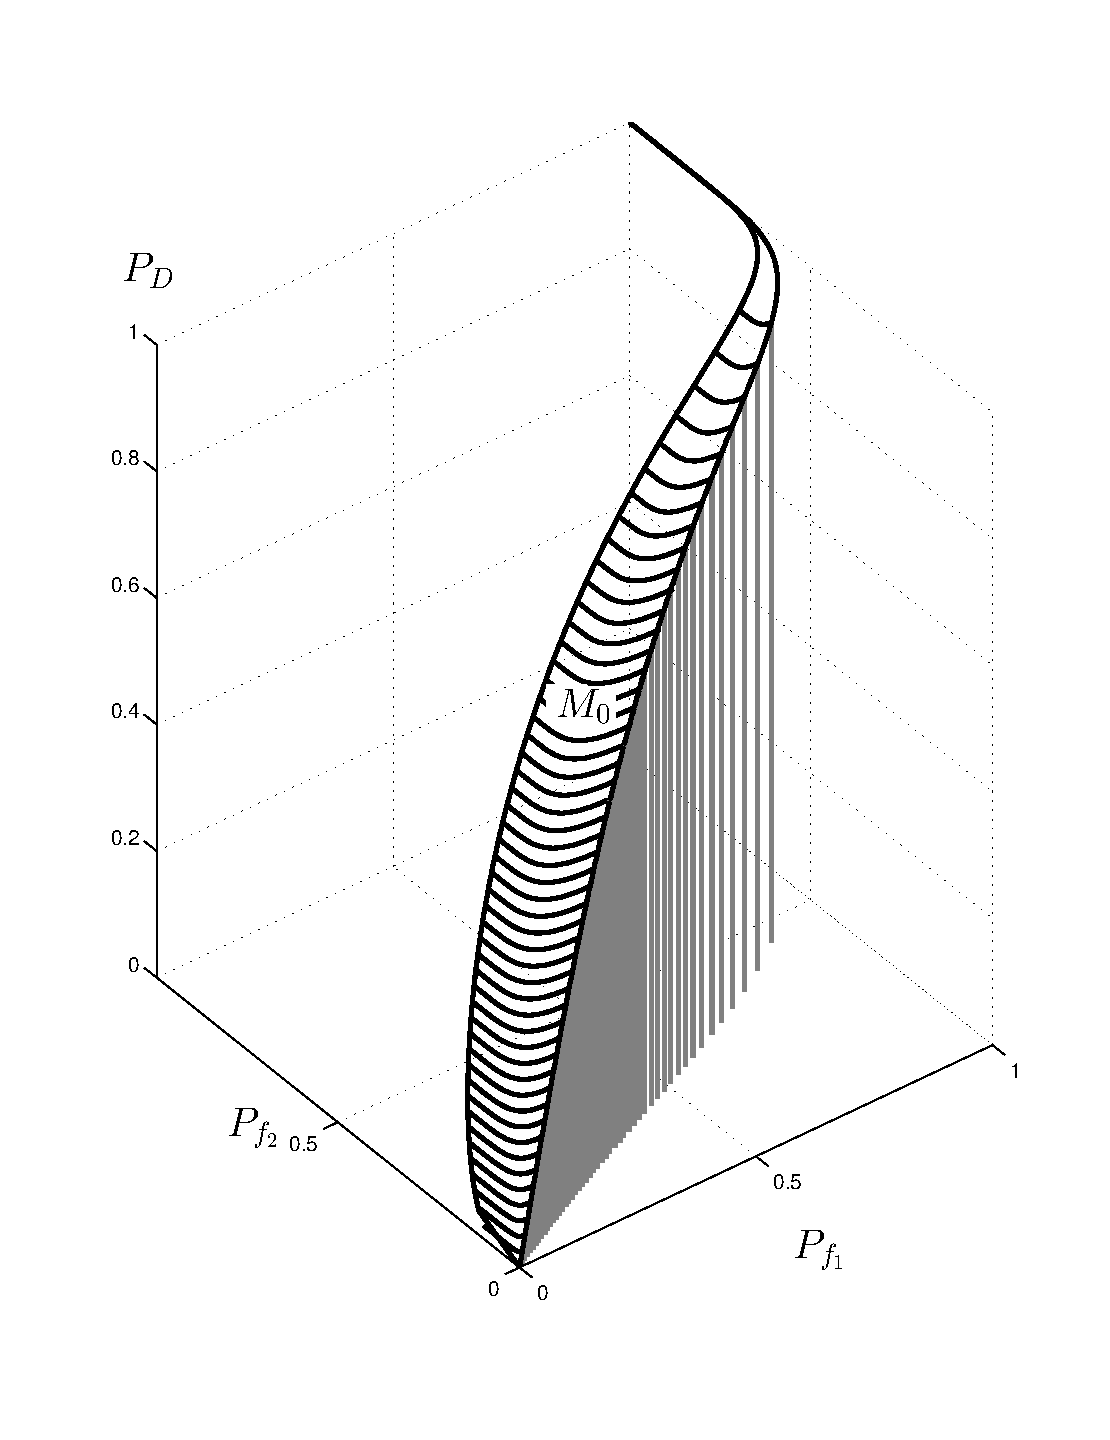
\includegraphics[width=12cm]{singleROC.eps}
\caption{Region that can be achieved by Neyman Pearson testing with $k_i \geq 0 (i=1, ..., M)$.}
\label{pic: surface for m0 gaussian}
\end{figure}
\newpage

\begin{figure}[!t]
\centering
\includegraphics[width=12cm]{singlecontour.eps}
\caption{Region that can be achieved by Neyman Pearson testing with $k_i \geq 0 (i=1, ..., M)$.}
\label{pic: contour for m0 gaussian}
\end{figure}

\begin{figure}[!t]
\centering
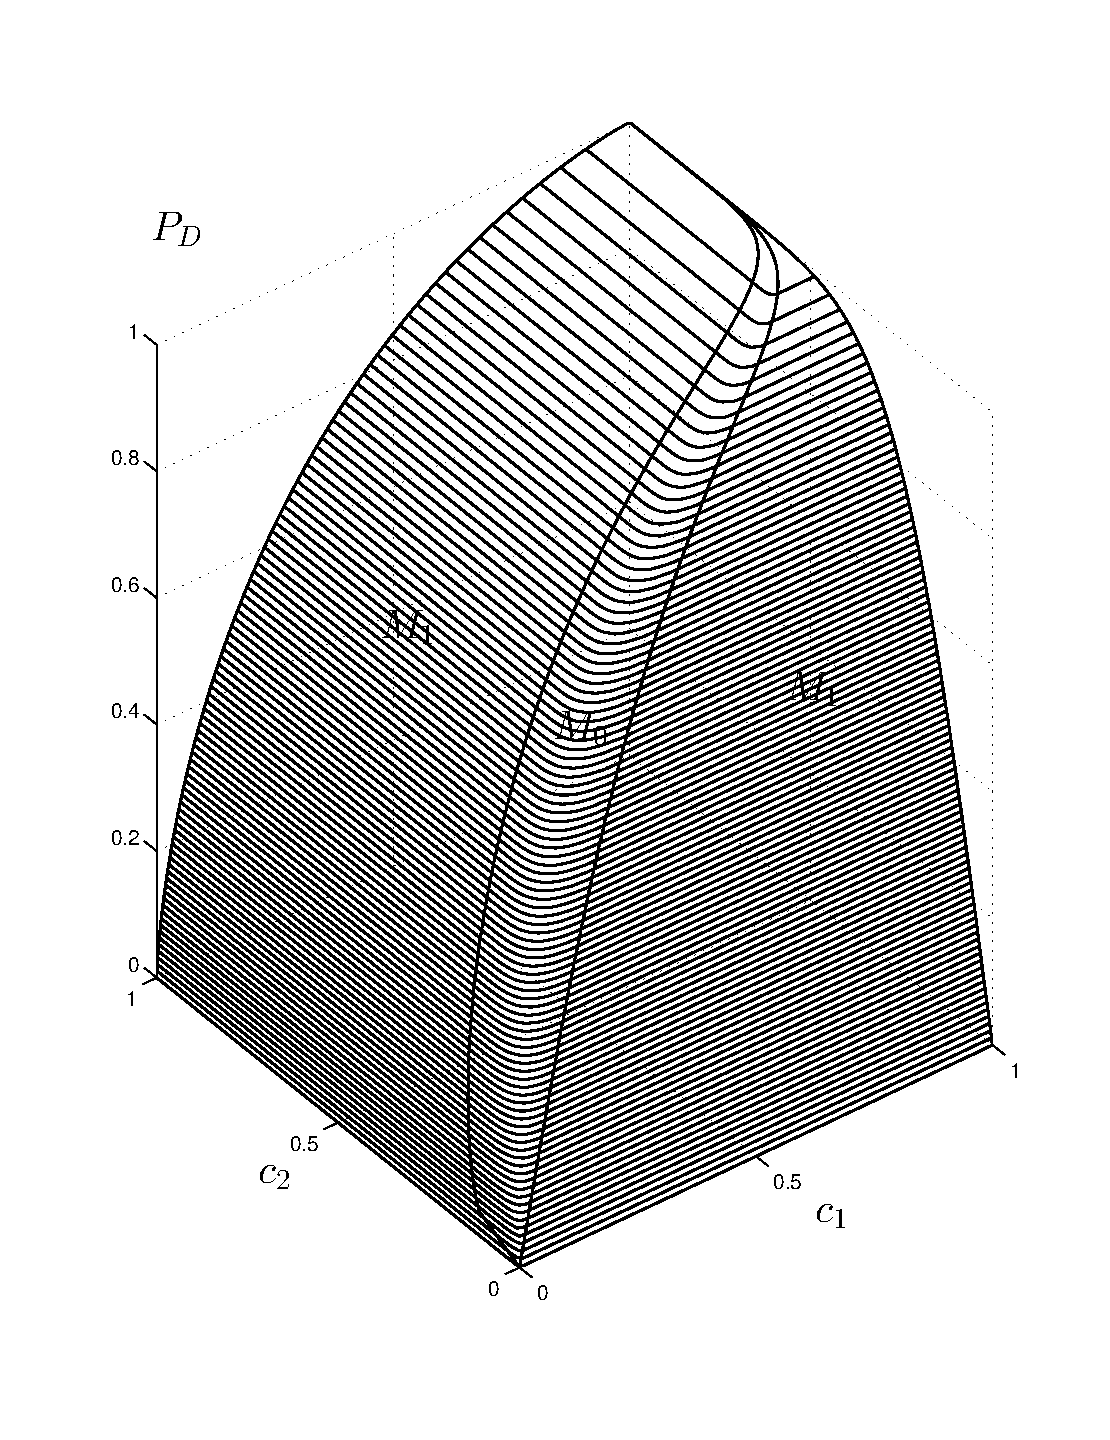
\includegraphics[width=12cm]{ROC2.eps}
\caption{The M-ROC surface for Gaussian Hypotheses.}
\label{pic: LJS}
\end{figure}

\begin{figure}[!t]
\centering
\includegraphics[width=12cm]{LJcontour.eps}
\caption{Contour for M-ROC surface.}
\label{pic: LJS contour}
\end{figure}


\begin{figure}[!t]
\centering
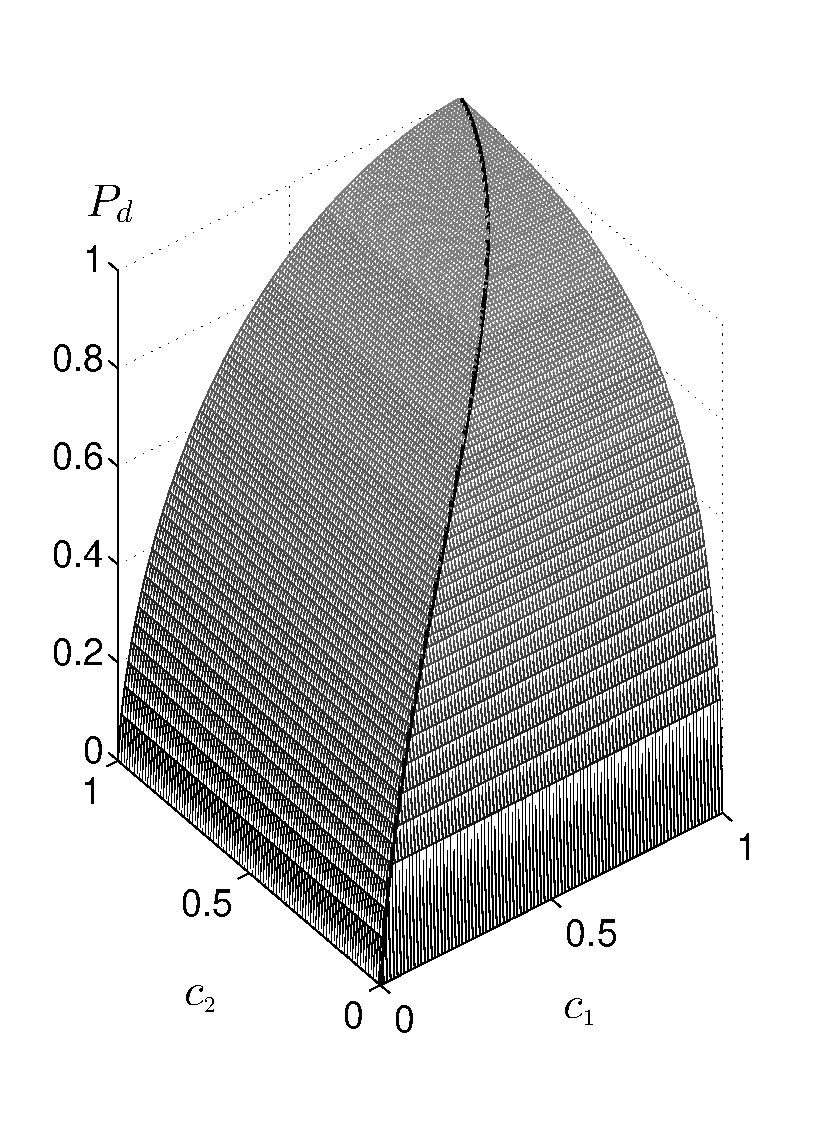
\includegraphics[width=12cm]{simu_chi2ROC.eps}
\caption{The M-ROC for the Chi-square example.}
\label{pic: LJS for chisquare}
\end{figure}


\begin{figure}[!t]
\centering
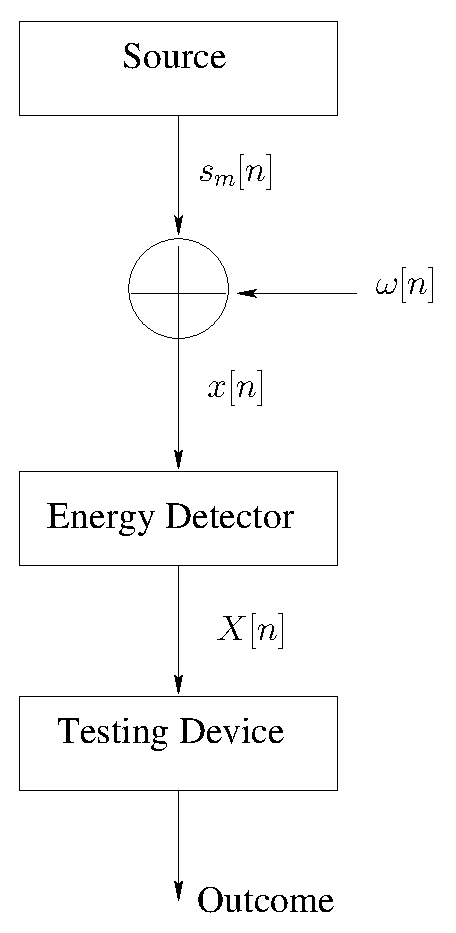
\includegraphics[width=8cm]{fig1.eps}
\caption{The Block Diagram for Energy Based Spectrum Sensing.}
\label{pic: block diagram}
\end{figure}

\begin{figure}[!t]
\centering
\includegraphics[width=12cm]{PFchange.eps}
\caption{Change of $P_{f_1}$ and $P_{f_2}$ after each iteration.}
\label{pic: PFchange}
\end{figure}

\begin{figure}[!t]
\centering
\includegraphics[width=12cm]{PDchange.eps}
\caption{Change of $P_d$ after each iteration.}
\label{pic: PDchange}
\end{figure}

\begin{figure}[!t]
\centering
\includegraphics[width=12cm]{mini.eps}
\caption{ROC for minimax decision rule.}
\label{pic: minimax}
\end{figure}

\end{spacing}
\end{document}
